\documentclass[aoas,preprint]{imsart}

\usepackage[OT1]{fontenc}
\usepackage{amsmath}
\usepackage{natbib}
\usepackage[colorlinks,citecolor=blue,urlcolor=blue]{hyperref}
\usepackage{bm}
\usepackage{graphicx}

% settings
\pubyear{2016}
\volume{0}
\issue{0}
\firstpage{1}
\lastpage{14}

\startlocaldefs
\numberwithin{equation}{section}
\endlocaldefs
\bibliographystyle{imsart-nameyear}

\begin{document}

\begin{frontmatter}
\title{Supplementary Material\\Efficient estimation of age-specific social contact rates between men and women}
\runtitle{Supplementary Material}
\begin{aug}
\author{\fnms{Jan} \snm{van de Kassteele}},
\author{\fnms{Jan} \snm{van Eijkeren}}
\and
\author{\fnms{Jacco} \snm{Wallinga}}
\runauthor{J. van de Kassteele et al.}
\end{aug}
\end{frontmatter}

\section{Exploratory analyses}

We first explored the contact survey dataset. We tested for differences in the number of participants by day of the week. No evidence was found for any differences (chi-squared test, p-value = 0.96), implying that no weighing procedures had to be applied.

In total, 351 participants declared they had missed one or more contacts. These contacts are missing because the participant forgot to report them, or there were too many contacts to report them all. More specifically, 200 participants had missed 1-4 contacts, 71 participants had missed 5-9 contacts, and 80 participants had missed 10 or more contacts. No evidence was found for an association between number of missed contacts and the participants' age (10-year age groups, chi-square test, p-value = 0.30), nor with the participants' sex (p-value = 0.44). This indicates that, up to a proportionally constant, the reported number of contacts provides a good proxy for the true number of contacts.

To develop some insight in the number of and variability in the reported contacts, Figure 1 shows boxplots of crude number of contacts per day as reported by the participants, stratified by 10-year age groups and the participant's sex, calculated using equation (2.1) (main text). Contact intensities are highly variable and differ by age and sex. Especially women in the age category 20 - 30 report more contacts than men in 
the same age category.

\begin{figure}
\centering
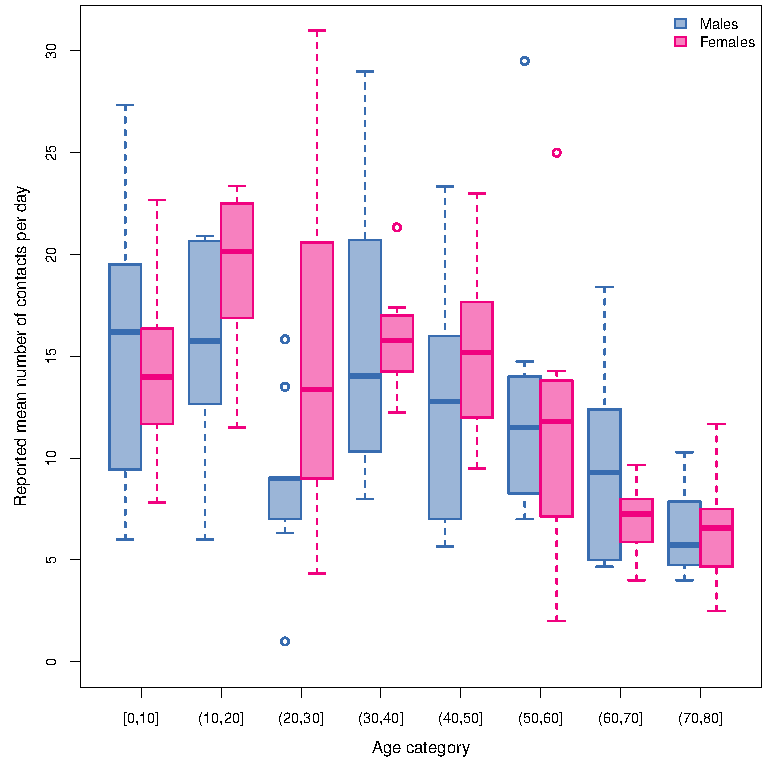
\includegraphics{fig_mean_number_of_contacts.pdf}
\caption{Boxplots of the crude number of contacts per day as reported by the participants, stratified by 10-year age groups and the participant's.}
\end{figure}

To assess the validity of the assumption of a Negative Binomial distribution for the total number of contacts (conditional on its mean and dispersion parameter), we calculated the mean and variance of the total number of contacts stratified by 10-year age groups and sex of both the participants and contacts. Because the variance of a Negative Binomial distribution is a quadratic function of the expectation, the standard deviation plotted against the expectation should be on a straight line. Based on visual inspection, the assumption of a Negative Binomial distribution for the total number of contacts seems legitimate.

\section{Data pre-processing}

We start with three datasets: the participant data (\texttt{part.data}), the contact data (\texttt{cont.data}), and the population data (\texttt{pop.data}). The participant data contains the participant's unique ID number, age and sex (\texttt{local.id, part.age, part.sex}). The contact data contains for each participant's ID, the reported contact's age and sex (\texttt{local.id, cont.age, cont.sex}). The population data contains the population numbers by age and sex (\texttt{cont.age, cont.sex, pop}), linked to the contact as required in section 2.1 (main text).

\texttt{part.data} and \texttt{cont.data} are merged into one dataset \texttt{polymod.data}. The total number of contacts of any age and sex-specific combination is found by cross tabulation of the participant ID's in \texttt{polymod.data}, stratified by participant age, contact age, participant sex and contact sex (\texttt{polymod.cont.tab}). The total number of participants of any age and sex-specific combination is found by cross tabulation of the number of unique participant ID’s, stratified by participant age and sex (\texttt{polymod.part.tab}). These are merged with \texttt{pop.data}, resulting in one large dataset \texttt{polymod.tab}, resulting in $(81 \times 2)^2 = 26,244$ records.

The records are sorted by contact sex, within contact sex by participant sex, within participant sex by contact age, and within contact age by participant age. Hence, records 1 to 6,561 contain the male-to-male contact data, records 6,562 to 13,122 the female-to-male contact data, records 13,123 to 19,683 the male-to-female contact data and records 19,684 to 26,244 the female-to-female contact data. The R-code is showed below.

\begin{verbatim}
#
# Data preprocessing
#

# Merge part.data and cont.data into polymod.data
polymod.data <- merge(part.data, cont.data, all = TRUE)

# Set age range
age <- 0:80; n <- length(age)

# Make age a categorical variable (needed for cross tabulation)
polymod.data <- within(polymod.data, {
  part.age <- factor(part.age, levels = age)
  cont.age <- factor(cont.age, levels = age)
})

#
# Cross tabulation
#

# Cross tabulate number of participants for each combination of age and sex
# t = number of participants
polymod.part.tab <- with(subset(polymod.data, !duplicated(local.id)),
  as.data.frame(table(
    part.age = part.age, part.sex = part.sex),
    responseName = "t"))
# Cross tabulate number of contacts for each combination of age and sex
# y = number of participants x number of contacts
polymod.cont.tab <- with(polymod.data,
  as.data.frame(table(
    part.age = part.age, cont.age = cont.age,
    part.sex = part.sex, cont.sex = cont.sex),
    responseName = "y"))

# Make age an integer again
polymod.part.tab <- within(polymod.part.tab, {
  part.age <- as.numeric(as.character(part.age))
})
polymod.cont.tab <- within(polymod.cont.tab, {
  part.age <- as.numeric(as.character(part.age))
  cont.age <- as.numeric(as.character(cont.age))
})

# Merge polymod.cont.tab, polymod.part.tab and pop.data
# polymod.tab is the tabulated version of polymod.data
polymod.tab <- merge(polymod.part.tab,
  merge(polymod.cont.tab, pop.data, all = TRUE), all = TRUE)

# Reorder polymod.tab
polymod.tab <- polymod.tab[c(
  "part.age", "cont.age",
  "part.sex", "cont.sex",
  "y", "t", "w")]
polymod.tab <- with(polymod.tab,
polymod.tab[order(cont.sex, part.sex, cont.age, part.age), ])

# Reorder pop.data
pop.data <- with(pop.data, pop.data[order(cont.sex, cont.age), ])

# Calculate denominator U = number of participants t x population w
# Divide by 1e6 for better numerical properties (inflates contact rate c)
# If t or w = 0, then set U = 1 and y = NA
# (record will not contribute to likelihood)
polymod.tab <- within(polymod.tab, {
  U <- t*w/1e6
  y <- ifelse(U == 0, yes = NA, no = y)
  U <- ifelse(U == 0, yes = 1, no = U)
})
\end{verbatim}

\section{Node IDs}

Specific node IDs of the Gaussian Markov Random Field prior have to specified (section 2.3, main text). For each matrix block of male-to-male ($\textit{MM}$), female-to-male ($\textit{FM}$), male-to-female ($\textit{MF}$) and female-to-female ($\textit{FF}$) a matrix is generated with zeroes as entries. Next, generate \texttt{LT1} and \texttt{LT2} as the Boolean representation of the lower triangular part of these matrices, respectively with and without diagonal. \texttt{nn1} and \texttt{nn2} are the number of \texttt{TRUE} entries in \texttt{LT1} and \texttt{LT2}. The lower triangular parts of the node matrices are filled first, then the upper triangular parts are filled by their transposed versions. Note that the triangular part of \texttt{node.FM} is filled by the transpose of \texttt{node.MF} and vice versa (Figure 1, main text). Finally, the node IDs are put together in one vector which is attached to the dataset containing the cross tabulated total number of contacts.

The R-code below is used to construct record IDs and node IDs, given $n$ age groups and a possible stratification to $sex$. For $\texttt{n = 5}$ and $\texttt{sex = TRUE}$, the record IDs and node IDs provides the numbers shown in Figure 1 (main text).

\begin{verbatim}
# Function to construct record IDs in matrix form
construct.recordID <- function(n, sex = TRUE) {
  if (sex) {
    # Sex specific
    rec.MM <- matrix(        1:n^2, nrow = n, ncol = n)
    rec.FM <- matrix(  n^2 + 1:n^2, nrow = n, ncol = n)
    rec.MF <- matrix(2*n^2 + 1:n^2, nrow = n, ncol = n)
    rec.FF <- matrix(3*n^2 + 1:n^2, nrow = n, ncol = n)
    return(list(rec.MM = rec.MM, rec.FM = rec.FM,
                rec.MF = rec.MF, rec.FF = rec.FF))
  } else {
    # Not sex specific
    rec <- matrix(1:n^2, nrow = n, ncol = n)
    return(list(rec = rec))
  }
}

# Function to construct node IDs in matrix form
construct.nodeID <- function(n, sex = TRUE) {
  if (sex) {
    # Sex specific
    nn1 <- n*(n + 1)/2 # Number of nodes in MM and FF
    nn2 <- n^2         # Number of nodes in FM and MF
    node.MM <- node.FF <- matrix(0, nrow = n, ncol = n) # Empty matrix
    LT <- lower.tri(node.MM, diag = TRUE) # Lower tri of MM and FF with diag
    node.MM[ LT] <- 1:nn1           # Fill lower tri with node IDs
    node.MM[!LT] <- t(node.MM)[!LT] # Fill upper tri with transposed
    node.FM      <- matrix(nn1 + 1:nn2, nrow = n, ncol = n) # Fill entire matrix
    node.MF      <- t(node.FM)                              # Transposed
    node.FF[ LT] <- nn1 + nn2 + 1:nn1 # As node.MM
    node.FF[!LT] <- t(node.FF)[!LT]
    return(list(node.MM = node.MM, node.FM = node.FM,
                node.MF = node.MF, node.FF = node.FF))
  } else {
    # Not sex specific
    nn <- n*(n + 1)/2
    node <- matrix(0, nrow = n, ncol = n)
    LT <- lower.tri(node, diag = TRUE)
    node[ LT] <- 1:nn
    node[!LT] <- t(node)[!LT]
    return(list(node = node))
  }
}

#
# Add node and record IDs to polymod.tab
#

# Node and record IDs
polymod.tab <- within(polymod.tab, {
  record.id <- with(construct.recordID(n, sex = TRUE),
    c(rec.MM, rec.FM, rec.MF, rec.FF))
  node.id <- with(construct.nodeID(n, sex = TRUE),
    c(node.MM, node.FM, node.MF, node.FF))
})
\end{verbatim}

\section{Construction of the R matrix}

The structure matrix $\bm{R}$ is constructed using the R package \texttt{Matrix} that allows us to work with large sparse matrices. We define a function to make difference matrices $\bm{D}_1$ and $\bm{D}_2$ for $n$ age classes (section 2.3). We can specify the order of the differences. Usually this is set to \texttt{order = 2}. Three matrices are defined which contain the row indices and column indices of $\bm{D}_1$ and $\bm{D}_2$ to keep if we are dealing with a triangular matrix (\texttt{tri = TRUE}). This is just a simple book keeping trick. Finally, the (reduced) $\bm{D}_1$ and $\bm{D}_2$ are stacked together in matrix $\bm{D}$.

\begin{verbatim}
# Function to construct D-matrix
construct.Dmat <- function(n, order, tri = FALSE) {
  In <- Diagonal(n)            # n x n matrix
  D0 <- diff(In, diff = order) # Differences for single vector
  D1 <- kronecker(In, D0)      # Differences in horizontal direction
  D2 <- kronecker(D0, In)      # Differences in   vertical direction
  if (tri) {
    # For lower triangular matrix (MM and FF)
    ri1.mat <- matrix(1:((n - order)*n), nrow = n - order, ncol = n)
    ri2.mat <- matrix(1:(n*(n - order)), nrow = n, ncol = n - order)
    ci.mat  <- matrix(1:n^2, nrow = n, ncol = n)
    ri1 <- ri1.mat[row(ri1.mat) >=  col(ri1.mat)         ] # Rows to keep in D1
    ri2 <- ri2.mat[row(ri2.mat) >= (col(ri2.mat) + order)] # Rows to keep in D2
    ci  <-  ci.mat[row(ci.mat)  >=  col(ci.mat)          ] # Cols to keep in D1&D2
    D <- rBind(D1[ri1, ci], D2[ri2, ci])
    return(list(D0 = D0, D1 = D1, D2 = D2, ri1 = ri1, ri2 = ri2, ci = ci, D = D))
  } else {
    # For full matrix (FM)
    D <- rBind(D1, D2)
    return(list(D0 = D0, D1 = D1, D2 = D2, D = D))
  }
}
\end{verbatim}

The function above is called for each matrix \textit{MM}, \textit{FM} and \textit{FF}. The $\bm{R}$ matrix is obtained by calculating $\bm{D}^\text{T}\bm{D}$. By setting \texttt{sex = TRUE}, we obtain sex specific $\bm{R}$ matrices.

\begin{verbatim}
# Function to construct R-matrix
construct.Rmat <- function(n, order = 2, sex = TRUE) {
  if (sex) {
    # Sex specific
    D.MM <- D.FF <- construct.Dmat(n, order, tri = TRUE )$D # MM and FF
    D.FM         <- construct.Dmat(n, order, tri = FALSE)$D # FM
    D <- bdiag(D.MM, D.FM, D.FF) # Block diagonal difference matrix D
    R <- crossprod(D)            # Structure matrix R
    R <- as(R, "dsCMatrix")      # R is symmetric sparse column compressed matrix
    return(list(D = D, R = R))
  } else {
    # Not sex specific
    D <- construct.Dmat(n, order, tri = TRUE)$D
    R <- crossprod(D)
    R <- as(R, "dsCMatrix")
    return(list(D = D, R = R))
  }
}

# Construct structure matrix R (RW2 prior)
R <- construct.Rmat(n, order = 2, sex = TRUE)$R
\end{verbatim}

\section{Running the model with INLA}

The statistical model is specified and fitted using the \texttt{inla} function from the R package \texttt{INLA}. The response variable is the total number of contacts \texttt{y}. The likelihood of the response variable is a Negative Binomial. The logarithm of the expectation is described by a constant term plus a GMRF term. The nodes are represented by the \texttt{node.id} vector. The model is a generic model with structure matrix \texttt{R}. Its rank deficiency is $3 \times \texttt{order}^2 = 12$ (\texttt{order = 2}) and a sum-to-zero constraint is put on the values of \texttt{x}. To prevent numerical instabilities, the diagonal of \texttt{R} is set to a low value, here $10^{-3}$. The prior for the precision parameter $\tau$ is a gamma prior, here with shape and rate parameter 1 and 0.0001. The denominator $U$ is specified by \texttt{E}. The tabulated dataset is called \texttt{polymod.tab}. A Gaussian prior with mean 0 and precision 0.001 is set to the intercept $\beta$. A Gaussian prior with mean 0 and precision 0.001 is set to the log-dispersion parameter $\theta$. The linear predictor $\beta+\bm{x}$ is computed by setting \texttt{compute = TRUE}. Enabling computation of the WAIC is set by \texttt{waic = TRUE}, predictive measures by \texttt{cpo = TRUE}, and sampling from the joint posterior is enabled by \texttt{config = TRUE}. The last one is needed for calculating credible intervals.

\begin{verbatim}
#
# Model contact patterns with INLA
#

# Run model
polymod.mod <- inla(
  y ~ 1 + f(node.id, model = "generic0", Cmatrix = R,
    # log-Gamma(1, 0.0001) prior on log-precision
    hyper = list(prec = list(prior = "loggamma", param = c(1, 0.0001))),
    rankdef = 12, constr = TRUE, diagonal = 0.001),
  E = U,
  family = "nbinomial",
  data = polymod.tab,
  # Normal(0, 0.001) prior on intercept
  control.fixed = list(mean.intercept = 0, prec.intercept = 0.001),
  # Normal(0, 0.001) prior on log-dispersion parameter
  control.family = list(
    hyper = list(theta = list(prior = "gaussian", param = c(0, 0.001)))),
  # Compute linear predictor
  control.predictor = list(compute = TRUE, link = 1),
  control.compute = list(
    waic = TRUE,    # Compute WAIC
    cpo = TRUE,     # Compute cross-validated predictive measures
    config = TRUE)) # Enable posterior sampling
\end{verbatim}

The results are added to \texttt{polymod.tab}.

\begin{verbatim}
#
# Post processing
#

# Add expected c and m to polymod.tab
# c = exp(linear predictor) = contact rate
# m = w*c = number of contacts
polymod.tab <- within(polymod.tab, {
  # Divide c by 1e6 to go back to original scale (deflates contact rate c)
  c <- exp(polymod.mod$summary.linear.predictor$mean)/1e6
  m <- w*c
})
\end{verbatim}

\section{Aggregating contact intensities and rates}

In some occasions it may be useful to aggregate the estimated age and sex-specific contact intensities and rates into courser strata, like wider ages classes. The equations below can also be combined.

\subsection{Aggregation over sexes}
The mean number of individuals of age $j$ that are contacted by one male of age $i$ during one day is $m_\mathit{ij}^M = m_\mathit{ij}^\mathit{MM} + m_\mathit{ij}^\mathit{MF}$. The same applies to females. Since the sum $m_\mathit{ij}^M + m_\mathit{ij}^F$ represent one male plus one female, and the population numbers are sex dependent, a weighted average should be calculated:
\begin{equation}
m_\mathit{ij} = \frac{w_i^M (m_\mathit{ij}^\mathit{MM} +m_\mathit{ij}^\mathit{MF}) + w_i^F (m_\mathit{ij}^\mathit{FM}+m_\mathit{ij}^\mathit{FF})}{w_i^M+w_i^F }.
\end{equation}

\begin{figure}
\centering
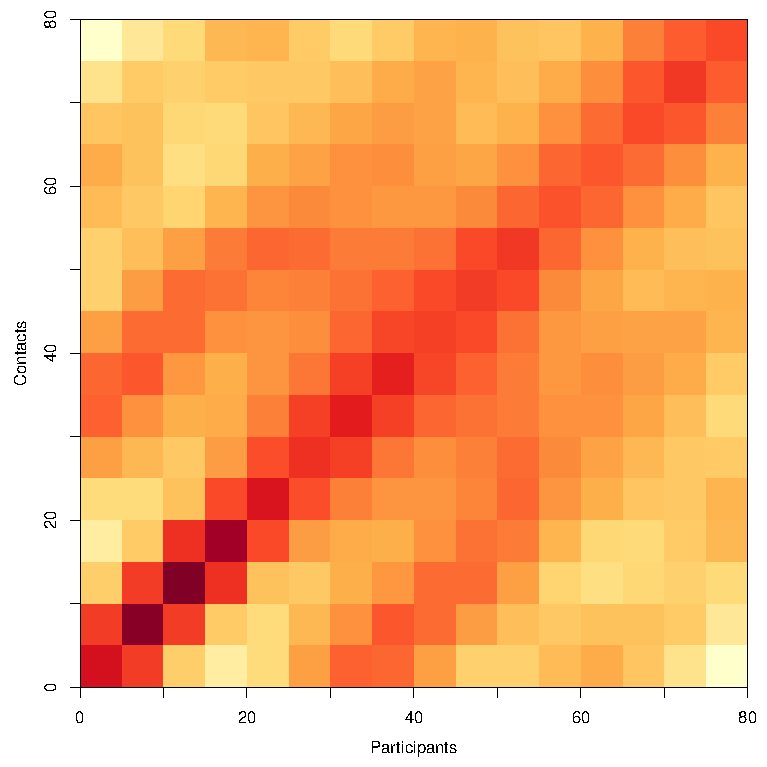
\includegraphics{fig_contact_matrix_aggregated.pdf}
\caption{Aggregated contact rates over both sexes by five year age groups. The horizontal axis gives the age of the participants; the vertical axis gives the age of the contacts. The color scale indicates the relative values of the contact rates from low (yellow) to high (red).}
\end{figure}

\subsection{Aggregation over ages}
A similar principle applies to aggregation over ages. Let us consider the \textit{MF} contacts for the moment. The mean number of female individuals in age class $\tilde{j}$ of consecutive ages $j \in J$ that are contacted by one male of age $i$ during one day is $m_\mathit{i\tilde{j}}^\mathit{MF} = \sum\limits_{j \in J} m_\mathit{ij}^\mathit{MF}$. We extend this to all males in age class $\tilde{i}$ of consecutive ages $i \in I$. Since the sum represents several males, and the male population numbers are age dependent, a weighted average should be calculated:
\begin{equation}
m_{\tilde{i}\tilde{j}}^\mathit{MF} = \frac{\sum\limits_{i \in I} w_i^M \sum\limits_{j \in J} m_\mathit{ij}^\mathit{MF}}{\sum\limits_{i \in I} w_i^M}.
\end{equation}
The relation fulfils the required symmetry $m_{\tilde{i}\tilde{j}}^\mathit{MF} w_{\tilde{i}}^M = m_{\tilde{j}\tilde{i}}^\mathit{FM} w_{\tilde{j}}^F$, where $w_{\tilde{i}}^M$ and $w_{\tilde{j}}^F$ are the sums of the population sizes of males of consecutive ages $i \in I$ and females of consecutive ages $j \in J$ respectively. Similar formulas apply to the \textit{MM}, \textit{FM} and \textit{FF} contacts. An application of both equations is shown in Figure 2. This figure shows the aggregated contact rates over both sexes by five year age groups. The R-code is given below.

\begin{verbatim}
#
# Aggregation of contact intensities and rates
#

# Set age range
age <- 0:80; n <- length(age)

# Define age cateogries
age.cat <- cut(x = age, breaks = seq(from = 0, to = 80, by = 5),
  include.lowest = TRUE, right = FALSE)

# Reshape pop.data in wide format. Sex is put in separate columns
pop.data <- cbind(
  data.frame(age = age),
  matrix(pop.data$w, nrow = n, ncol = 2,
    dimnames = list(NULL, c("wM", "wF"))))
pop.data <- within(pop.data, w <- wM + wF)

# Create a dataframe contact.data with n^2 rows. Sex is put in separate columns
contact.data <- cbind(
  expand.grid(part.age = age, cont.age = age),
  matrix(polymod.tab$c, nrow = n^2, ncol = 4,
    dimnames = list(NULL, c("cMM", "cFM", "cMF", "cFF"))),
  matrix(polymod.tab$m, nrow = n^2, ncol = 4,
    dimnames = list(NULL, c("mMM", "mFM", "mMF", "mFF"))))

#
# Aggregate over sexes (equation 6.1)
#

# Aggregate contact intensities over sexes 
record.id.part <- match(x = contact.data$part.age, table = pop.data$age)
contact.data <- within(contact.data, {
  m <- (pop.data[record.id.part, "wM"]*(mMM + mMF) +
    pop.data[record.id.part, "wF"]*(mFM + mFF))/pop.data[record.id.part, "w"]
})

# Calculate contact rates
record.id.cont <- match(x = contact.data$cont.age, table = pop.data$age)
contact.data <- within(contact.data, {
  wM <- pop.data[record.id.cont, "wM"]
  wF <- pop.data[record.id.cont, "wF"]
  w  <- pop.data[record.id.cont, "w"]
  c <- m/w
})

# Reorder columns
contact.data <- contact.data[, c(
  "part.age", "cont.age",
  "wM", "wF", "w",
  "mMM", "mFM", "mMF", "mFF", "m",
  "cMM", "cFM", "cMF", "cFF", "c")]

#
# Aggregate over ages (equation 6.2)
#

# Add age categories to contact.data and pop.data
contact.data <- cbind(contact.data,
  expand.grid(part.age.cat = age.cat, cont.age.cat = age.cat))
pop.data <- cbind(pop.data, age.cat = age.cat)

# Aggregate population numbers
pop.data.agg <- aggregate(cbind(wM, wF, w) ~ age.cat,
  FUN = sum, data = pop.data)

# Aggegrate contact intensities over ages
record.id.part.agg <- match(
  x = contact.data$part.age.cat, table = pop.data.agg$age.cat)
contact.data.agg <- within(contact.data, {
  m   <- pop.data[record.id.part, "w" ]*m  /pop.data.agg[record.id.part.agg, "w" ]
  mMM <- pop.data[record.id.part, "wM"]*mMM/pop.data.agg[record.id.part.agg, "wM"]
  mFM <- pop.data[record.id.part, "wF"]*mFM/pop.data.agg[record.id.part.agg, "wF"]
  mMF <- pop.data[record.id.part, "wM"]*mMF/pop.data.agg[record.id.part.agg, "wM"]
  mFF <- pop.data[record.id.part, "wF"]*mFF/pop.data.agg[record.id.part.agg, "wF"]
})
contact.data.agg <- aggregate(
  cbind(mMM, mFM, mMF, mFF, m) ~ part.age.cat + cont.age.cat,
  FUN = sum, data = contact.data.agg)

# Calculate contact rates
record.id.cont.agg <- match(
  x = contact.data.agg$cont.age.cat, table = pop.data.agg$age.cat)
contact.data.agg <- within(contact.data.agg, {
  wM <- pop.data.agg[record.id.cont.agg, "wM"]
  wF <- pop.data.agg[record.id.cont.agg, "wF"]
  w  <- pop.data.agg[record.id.cont.agg, "w" ]
  cMM <- mMM/wM
  cFM <- mFM/wM
  cMF <- mMF/wF
  cFF <- mFF/wF
  c   <- m  /w
})

# Reorder columns
contact.data.agg <- contact.data.agg[, c(
  "part.age.cat", "cont.age.cat",
  "wM", "wF", "w",
  "mMM", "mFM", "mMF", "mFF", "m",
  "cMM", "cFM", "cMF", "cFF", "c")]
\end{verbatim}

\section{Table with contact intensities and contact rates}

The estimated mean numbers of contacts prove useful for parameterizing mathematical transmission models that are used in planning for, and evaluation of, intervention measures against respiratory infections. We provide the estimates in the file \texttt{contact\_matrix\_data.txt}. The file consists of 26,244 rows and nine columns:
\begin{enumerate}
\item Record ID
\item Node ID
\item Age of participant (0 - 80)
\item Age of contact (0 - 80)
\item Sex of participant
\item Sex of contact
\item Population number $w$ (linked to age and sex of contact)
\item Contact intensity $m$
\item Contact rate $c$ (per $10^6$)
\end{enumerate}

\end{document}
